% Created by tikzDevice version 0.12.3.1 on 2022-09-12 13:44:44
% !TEX encoding = UTF-8 Unicode
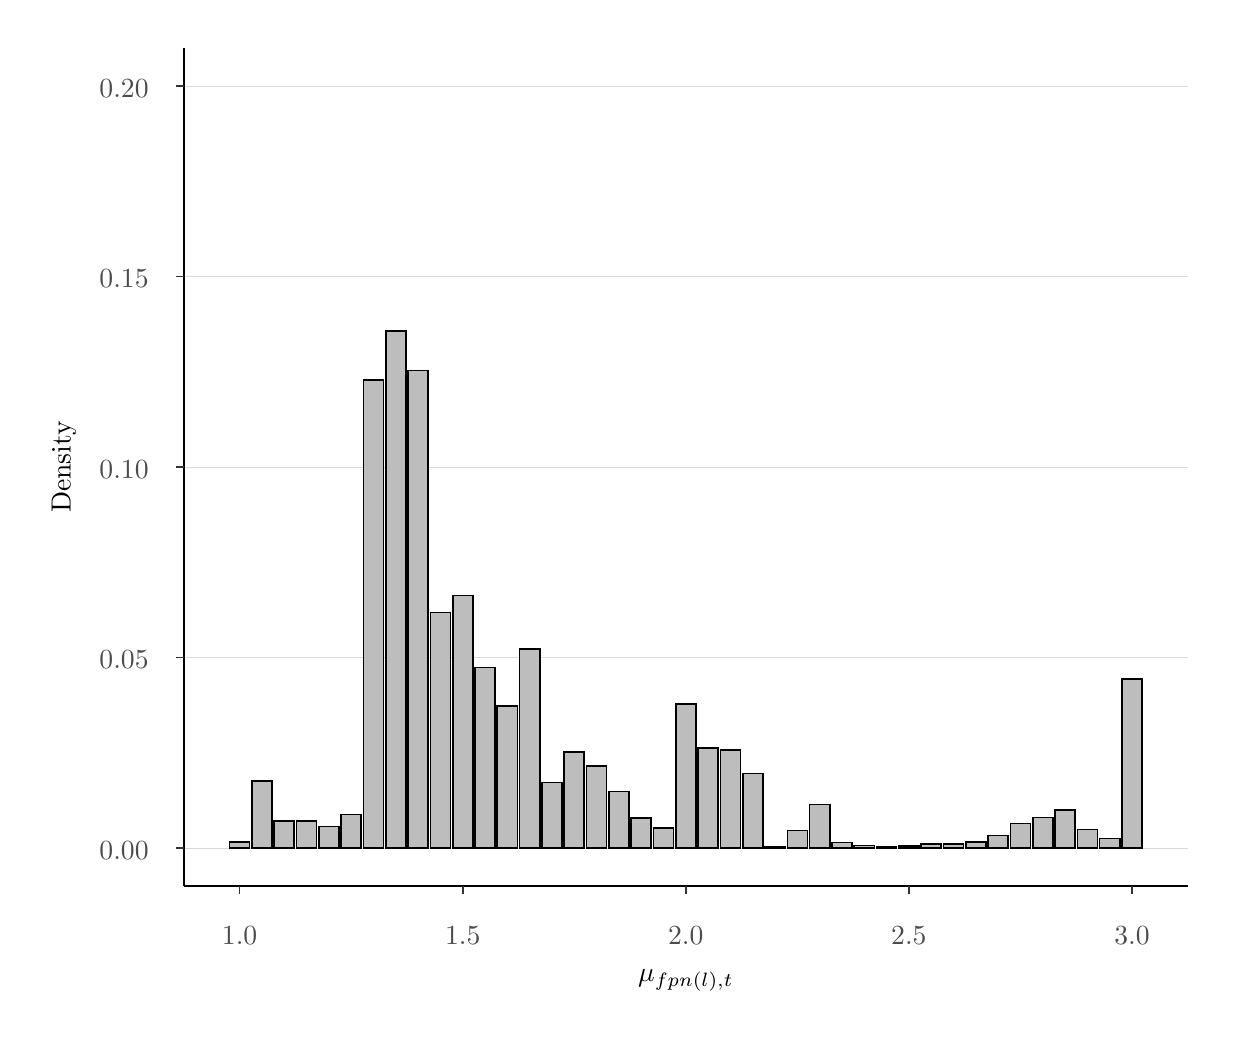
\begin{tikzpicture}[x=1pt,y=1pt]
\definecolor{fillColor}{RGB}{255,255,255}
\path[use as bounding box,fill=fillColor,fill opacity=0.00] (0,0) rectangle (433.62,361.35);
\begin{scope}
\path[clip] (  0.00,  0.00) rectangle (433.62,361.35);
\definecolor{drawColor}{RGB}{255,255,255}
\definecolor{fillColor}{RGB}{255,255,255}

\path[draw=drawColor,line width= 0.6pt,line join=round,line cap=round,fill=fillColor] ( -0.00,  0.00) rectangle (433.62,361.35);
\end{scope}
\begin{scope}
\path[clip] ( 56.47, 51.15) rectangle (419.17,354.12);
\definecolor{drawColor}{RGB}{255,255,255}

\path[draw=drawColor,line width= 0.3pt,line join=round] ( 56.47, 99.35) --
	(419.17, 99.35);

\path[draw=drawColor,line width= 0.3pt,line join=round] ( 56.47,168.21) --
	(419.17,168.21);

\path[draw=drawColor,line width= 0.3pt,line join=round] ( 56.47,237.07) --
	(419.17,237.07);

\path[draw=drawColor,line width= 0.3pt,line join=round] ( 56.47,305.92) --
	(419.17,305.92);

\path[draw=drawColor,line width= 0.3pt,line join=round] (116.89, 51.15) --
	(116.89,354.12);

\path[draw=drawColor,line width= 0.3pt,line join=round] (197.51, 51.15) --
	(197.51,354.12);

\path[draw=drawColor,line width= 0.3pt,line join=round] (278.12, 51.15) --
	(278.12,354.12);

\path[draw=drawColor,line width= 0.3pt,line join=round] (358.74, 51.15) --
	(358.74,354.12);
\definecolor{drawColor}{gray}{0.85}

\path[draw=drawColor,line width= 0.1pt,line join=round] ( 56.47, 64.92) --
	(419.17, 64.92);

\path[draw=drawColor,line width= 0.1pt,line join=round] ( 56.47,133.78) --
	(419.17,133.78);

\path[draw=drawColor,line width= 0.1pt,line join=round] ( 56.47,202.64) --
	(419.17,202.64);

\path[draw=drawColor,line width= 0.1pt,line join=round] ( 56.47,271.49) --
	(419.17,271.49);

\path[draw=drawColor,line width= 0.1pt,line join=round] ( 56.47,340.35) --
	(419.17,340.35);
\definecolor{drawColor}{RGB}{0,0,0}
\definecolor{fillColor}{gray}{0.74}

\path[draw=drawColor,line width= 0.6pt,line cap=rect,fill=fillColor] ( 72.95, 64.92) rectangle ( 80.21, 67.13);

\path[draw=drawColor,line width= 0.6pt,line cap=rect,fill=fillColor] ( 81.01, 64.92) rectangle ( 88.27, 89.09);

\path[draw=drawColor,line width= 0.6pt,line cap=rect,fill=fillColor] ( 89.08, 64.92) rectangle ( 96.33, 74.76);

\path[draw=drawColor,line width= 0.6pt,line cap=rect,fill=fillColor] ( 97.14, 64.92) rectangle (104.39, 74.76);

\path[draw=drawColor,line width= 0.6pt,line cap=rect,fill=fillColor] (105.20, 64.92) rectangle (112.45, 72.65);

\path[draw=drawColor,line width= 0.6pt,line cap=rect,fill=fillColor] (113.26, 64.92) rectangle (120.52, 77.04);

\path[draw=drawColor,line width= 0.6pt,line cap=rect,fill=fillColor] (121.32, 64.92) rectangle (128.58,234.00);

\path[draw=drawColor,line width= 0.6pt,line cap=rect,fill=fillColor] (129.38, 64.92) rectangle (136.64,251.84);

\path[draw=drawColor,line width= 0.6pt,line cap=rect,fill=fillColor] (137.45, 64.92) rectangle (144.70,237.44);

\path[draw=drawColor,line width= 0.6pt,line cap=rect,fill=fillColor] (145.51, 64.92) rectangle (152.76,149.99);

\path[draw=drawColor,line width= 0.6pt,line cap=rect,fill=fillColor] (153.57, 64.92) rectangle (160.83,156.13);

\path[draw=drawColor,line width= 0.6pt,line cap=rect,fill=fillColor] (161.63, 64.92) rectangle (168.89,130.18);

\path[draw=drawColor,line width= 0.6pt,line cap=rect,fill=fillColor] (169.69, 64.92) rectangle (176.95,116.13);

\path[draw=drawColor,line width= 0.6pt,line cap=rect,fill=fillColor] (177.76, 64.92) rectangle (185.01,136.78);

\path[draw=drawColor,line width= 0.6pt,line cap=rect,fill=fillColor] (185.82, 64.92) rectangle (193.07, 88.57);

\path[draw=drawColor,line width= 0.6pt,line cap=rect,fill=fillColor] (193.88, 64.92) rectangle (201.13, 99.71);

\path[draw=drawColor,line width= 0.6pt,line cap=rect,fill=fillColor] (201.94, 64.92) rectangle (209.20, 94.55);

\path[draw=drawColor,line width= 0.6pt,line cap=rect,fill=fillColor] (210.00, 64.92) rectangle (217.26, 85.33);

\path[draw=drawColor,line width= 0.6pt,line cap=rect,fill=fillColor] (218.06, 64.92) rectangle (225.32, 75.81);

\path[draw=drawColor,line width= 0.6pt,line cap=rect,fill=fillColor] (226.13, 64.92) rectangle (233.38, 72.23);

\path[draw=drawColor,line width= 0.6pt,line cap=rect,fill=fillColor] (234.19, 64.92) rectangle (241.44,117.04);

\path[draw=drawColor,line width= 0.6pt,line cap=rect,fill=fillColor] (242.25, 64.92) rectangle (249.51,101.06);

\path[draw=drawColor,line width= 0.6pt,line cap=rect,fill=fillColor] (250.31, 64.92) rectangle (257.57,100.38);

\path[draw=drawColor,line width= 0.6pt,line cap=rect,fill=fillColor] (258.37, 64.92) rectangle (265.63, 91.84);

\path[draw=drawColor,line width= 0.6pt,line cap=rect,fill=fillColor] (266.44, 64.92) rectangle (273.69, 65.42);

\path[draw=drawColor,line width= 0.6pt,line cap=rect,fill=fillColor] (274.50, 64.92) rectangle (281.75, 71.24);

\path[draw=drawColor,line width= 0.6pt,line cap=rect,fill=fillColor] (282.56, 64.92) rectangle (289.81, 80.67);

\path[draw=drawColor,line width= 0.6pt,line cap=rect,fill=fillColor] (290.62, 64.92) rectangle (297.88, 66.91);

\path[draw=drawColor,line width= 0.6pt,line cap=rect,fill=fillColor] (298.68, 64.92) rectangle (305.94, 65.83);

\path[draw=drawColor,line width= 0.6pt,line cap=rect,fill=fillColor] (306.74, 64.92) rectangle (314.00, 65.52);

\path[draw=drawColor,line width= 0.6pt,line cap=rect,fill=fillColor] (314.81, 64.92) rectangle (322.06, 65.67);

\path[draw=drawColor,line width= 0.6pt,line cap=rect,fill=fillColor] (322.87, 64.92) rectangle (330.12, 66.29);

\path[draw=drawColor,line width= 0.6pt,line cap=rect,fill=fillColor] (330.93, 64.92) rectangle (338.19, 66.31);

\path[draw=drawColor,line width= 0.6pt,line cap=rect,fill=fillColor] (338.99, 64.92) rectangle (346.25, 66.98);

\path[draw=drawColor,line width= 0.6pt,line cap=rect,fill=fillColor] (347.05, 64.92) rectangle (354.31, 69.44);

\path[draw=drawColor,line width= 0.6pt,line cap=rect,fill=fillColor] (355.12, 64.92) rectangle (362.37, 73.74);

\path[draw=drawColor,line width= 0.6pt,line cap=rect,fill=fillColor] (363.18, 64.92) rectangle (370.43, 76.00);

\path[draw=drawColor,line width= 0.6pt,line cap=rect,fill=fillColor] (371.24, 64.92) rectangle (378.49, 78.66);

\path[draw=drawColor,line width= 0.6pt,line cap=rect,fill=fillColor] (379.30, 64.92) rectangle (386.56, 71.62);

\path[draw=drawColor,line width= 0.6pt,line cap=rect,fill=fillColor] (387.36, 64.92) rectangle (394.62, 68.37);

\path[draw=drawColor,line width= 0.6pt,line cap=rect,fill=fillColor] (395.42, 64.92) rectangle (402.68,125.96);
\end{scope}
\begin{scope}
\path[clip] (  0.00,  0.00) rectangle (433.62,361.35);
\definecolor{drawColor}{RGB}{0,0,0}

\path[draw=drawColor,line width= 0.6pt,line join=round] ( 56.47, 51.15) --
	( 56.47,354.12);
\end{scope}
\begin{scope}
\path[clip] (  0.00,  0.00) rectangle (433.62,361.35);
\definecolor{drawColor}{gray}{0.30}

\node[text=drawColor,anchor=base east,inner sep=0pt, outer sep=0pt, scale=  1.00] at ( 43.72, 60.79) {0.00};

\node[text=drawColor,anchor=base east,inner sep=0pt, outer sep=0pt, scale=  1.00] at ( 43.72,129.65) {0.05};

\node[text=drawColor,anchor=base east,inner sep=0pt, outer sep=0pt, scale=  1.00] at ( 43.72,198.51) {0.10};

\node[text=drawColor,anchor=base east,inner sep=0pt, outer sep=0pt, scale=  1.00] at ( 43.72,267.36) {0.15};

\node[text=drawColor,anchor=base east,inner sep=0pt, outer sep=0pt, scale=  1.00] at ( 43.72,336.22) {0.20};
\end{scope}
\begin{scope}
\path[clip] (  0.00,  0.00) rectangle (433.62,361.35);
\definecolor{drawColor}{gray}{0.20}

\path[draw=drawColor,line width= 0.6pt,line join=round] ( 53.72, 64.92) --
	( 56.47, 64.92);

\path[draw=drawColor,line width= 0.6pt,line join=round] ( 53.72,133.78) --
	( 56.47,133.78);

\path[draw=drawColor,line width= 0.6pt,line join=round] ( 53.72,202.64) --
	( 56.47,202.64);

\path[draw=drawColor,line width= 0.6pt,line join=round] ( 53.72,271.49) --
	( 56.47,271.49);

\path[draw=drawColor,line width= 0.6pt,line join=round] ( 53.72,340.35) --
	( 56.47,340.35);
\end{scope}
\begin{scope}
\path[clip] (  0.00,  0.00) rectangle (433.62,361.35);
\definecolor{drawColor}{RGB}{0,0,0}

\path[draw=drawColor,line width= 0.6pt,line join=round] ( 56.47, 51.15) --
	(419.17, 51.15);
\end{scope}
\begin{scope}
\path[clip] (  0.00,  0.00) rectangle (433.62,361.35);
\definecolor{drawColor}{gray}{0.20}

\path[draw=drawColor,line width= 0.6pt,line join=round] ( 76.58, 48.40) --
	( 76.58, 51.15);

\path[draw=drawColor,line width= 0.6pt,line join=round] (157.20, 48.40) --
	(157.20, 51.15);

\path[draw=drawColor,line width= 0.6pt,line join=round] (237.82, 48.40) --
	(237.82, 51.15);

\path[draw=drawColor,line width= 0.6pt,line join=round] (318.43, 48.40) --
	(318.43, 51.15);

\path[draw=drawColor,line width= 0.6pt,line join=round] (399.05, 48.40) --
	(399.05, 51.15);
\end{scope}
\begin{scope}
\path[clip] (  0.00,  0.00) rectangle (433.62,361.35);
\definecolor{drawColor}{gray}{0.30}

\node[text=drawColor,anchor=base,inner sep=0pt, outer sep=0pt, scale=  1.00] at ( 76.58, 30.14) {1.0};

\node[text=drawColor,anchor=base,inner sep=0pt, outer sep=0pt, scale=  1.00] at (157.20, 30.14) {1.5};

\node[text=drawColor,anchor=base,inner sep=0pt, outer sep=0pt, scale=  1.00] at (237.82, 30.14) {2.0};

\node[text=drawColor,anchor=base,inner sep=0pt, outer sep=0pt, scale=  1.00] at (318.43, 30.14) {2.5};

\node[text=drawColor,anchor=base,inner sep=0pt, outer sep=0pt, scale=  1.00] at (399.05, 30.14) {3.0};
\end{scope}
\begin{scope}
\path[clip] (  0.00,  0.00) rectangle (433.62,361.35);
\definecolor{drawColor}{RGB}{0,0,0}

\node[text=drawColor,anchor=base,inner sep=0pt, outer sep=0pt, scale=  1.00] at (237.82, 16.79) {$\mu_{fpn(l),t}$};
\end{scope}
\begin{scope}
\path[clip] (  0.00,  0.00) rectangle (433.62,361.35);
\definecolor{drawColor}{RGB}{0,0,0}

\node[text=drawColor,rotate= 90.00,anchor=base,inner sep=0pt, outer sep=0pt, scale=  1.00] at ( 15.49,202.64) {Density};
\end{scope}
\end{tikzpicture}
